\documentclass[12pt,a4paper]{article}
\usepackage[margin=1in]{geometry}
\usepackage{graphicx}   % for figures
\usepackage{amsmath}    % for \text{} in math & aligned equations
\usepackage{hyperref}   % clickable links
\usepackage{parskip}    % nicer paragraph spacing
\usepackage{amsfonts}
\title{Mechanics \& Control Test \\[2pt]\large Martian Mindset Application}
\author{Tersoo Samuel Awai}
\date{July 2025}

\begin{document}
\maketitle

\section{Mechanics}
This report contains my worked solutions for the first two mechanics exercises.
\subsection{Topology and Mobility Analysis}
%-----------------------------------------------------------------
\subsubsection*{Exercise 1 -- Topology}
A concise topological graph for the serial and parallel manipulators is shown
in Fig. \ref{fig:serial-graph}.  

\begin{figure}[htbp]
  \centering
  % 40 % of text width; keep aspect
  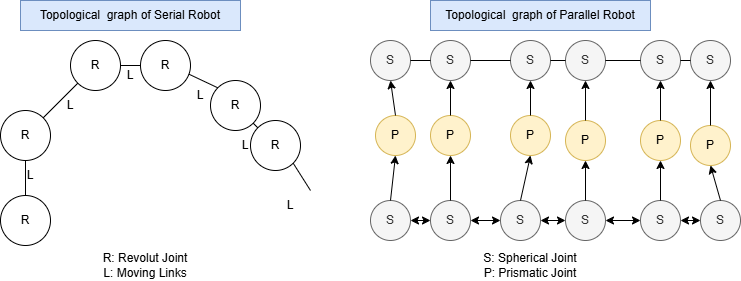
\includegraphics[width=0.9\linewidth]{../figs/topology.png}
  \caption{Topology diagram of the Serial Robot and Parallel Robot.}
  \label{fig:serial-graph}
\end{figure}



For background on graph‐based classification of
robot architectures, see Baron’s survey~\cite{Baron2008}.

%-----------------------------------------------------------------
\subsubsection*{Exercise 2 -- Mobility of Serial and Parallel Robots}

\text{Serial Robot:}
For a spatial mechanism with six motion parameters per link the Chebychev–Grübler–Kutzbach criterion can be implemented as follows:
\begin{equation}
m_s \;=\; 6\bigl(N - j - 1\bigr) \;+\; \sum_{i=1}^{j} f_i
       \;=\; 6(-c) \;+\; \sum_{i=1}^{j} f_i ,
\end{equation}
where \\ \(N\) is the number of links (including the ground) \\ 
\(j\) the number of joints\\ \(f_i\) the DOF of joint~\(i\) \\  
\(c = j + 1 - N\) counts \emph{independent} closed loops.



\[
N = 7 \; \rightarrow{6\text{ moving} + \text{base}} , \quad
j = 6, \quad
c = 0,\quad
\sum f_i = 6\times 1 = 6 .
\]
Hence
\[
m_s
      = 6\bigl(7-6-1\bigr) + 6 \;=\; 6 .
\]
Hence, the arm possesses the expected six spatial DOF.

\text{Simplified Formula:}
For an open \(n\)-joint serial chain there are \emph{no} independent
closed loops \((c = 0)\) and the number of links is \(N = j + 1\) ~\cite{Craig2005}.
Substituting these relations into Equation~(1)\footnote{%
CGK formula for spatial mechanisms:
\(m_s = 6(N-j-1) + \sum_{i=1}^{j} f_i\).} gives
\[
\boxed{\,m_s \;=\;
        \sum_{i=1}^{j} f_i\,},
\]
i.e.\ the mobility of a serial manipulator equals the sum of its joint
degrees of freedom.
%---------------------------------------------------------------
\text{Parallel Robot:}
Each leg is an \(S\!-\!P\!-\!S\) chain (one prismatic actuator between two
spherical joints):
\begin{align*}
&N = 14\;  \rightarrow{\text{base + platform} + 6\times 2\text{ rods})} \\
&j = 18\; \rightarrow{6\times 2S + 6\times 1P} \\
&\sum f_i = 6(3+1+3) = 42 .
\end{align*}
The mechanism closes \(c=6\) independent loops.  Therefore
\[
m_s^{\text{parallel}} \;=\; 6(-5) + 42 \;=\; 12 .
\]
This “12 DOF” value over-estimates the actual mobility because the
platform is \textit{statically over-constrained}.

\textbf{Redundancy correction:}
As shown by Merlet \cite[Sec.~2.2]{Merlet2006},
the CGK formula must subtract the directions \(r_k\) that
do not further restrict motion:
\begin{equation}
m_s \;=\; 6\,(N - j - 1) + \sum_{i=1}^{j} f_i
          \;-\; \sum_{k} r_k .
\end{equation}
For the SPS\(^6\) robot each leg contributes six redundant
constraint directions, so \(\sum_k r_k = 6\).
Hence
\[
m_s^{\text{Stewart}}
  = 12 - 6
  = 6 ,
\]
which matches physical reality.

\text{Loop-count alternative (same result):}
Equivalently, one may count the six independent closed kinematic loops
($c=6$—one per leg) and apply the loop form
\[
m_s = 6(-c) + \sum f_i = 6(-6) + 42 = 6 .
\]
Both approaches confirm the Stewart–Gough platform’s true mobility of
six spatial degrees of freedom.

\subsubsection*{Exercise 3 — When does CGK fail?  Classical counter-examples}

The Chebychev–Grübler–Kutzbach count
\[
m_s \;=\; 6\,(N-j-1)\;+\;\sum_{i=1}^{j}f_i
\]
assumes that every constraint introduced by every joint is \emph{independent}
and that the links behave as perfectly rigid bodies
\cite[Ch.~1]{Hunt1978}.  When those assumptions break down, the formula
can either under- or over-predict the true mobility.

\paragraph{(1) Over-constrained, paradoxical linkages.}
Bennett’s spatial 4R linkage has four revolute joints whose axes satisfy
specific skew-angle and offset conditions.
CGK yields
\[
m_s^{\text{CGK}} = 6\,(6-4-1)+4 = -2,
\]
yet the mechanism has \emph{one} genuine degree of freedom
\cite[Sec.~3.3.3]{Tsai1999}.  
The “missing” mobility arises because two constraint directions are
redundant; CGK counts them twice and predicts a negative value.

\paragraph{(2) Flexible-motion Sarrus linkage.}
Sarrus’s 6R parallel linkage comprises three pairs of opposite links
connected by revolute joints arranged in two parallel planes.
With \(N=7,\;j=6,\;f_i=1\), CGK returns
\[
m_s^{\text{CGK}} = 6\,(7-6-1)+6 = 0,
\]
yet the structure folds with \emph{one} DOF, forming a paradoxical
“motion-platform” without a prismatic joint
\cite[p.~148]{McCarthy2000}.  
Again, hidden constraint redundancies invalidate the independence
assumption.

From the above examples, it can be infered that while CGK is a powerful first-pass tool, it \text{does not always
work}.  Classic spatial linkages like Bennett’s and Sarrus’s provide
clear counter-examples where the naive count fails.

\newpage

\subsection{Geometry and Kinematics}
\subsubsection*{Exercise 4 -  Kinematics of 3DOF Robotic leg}

\text{Primitive Homogeneous Transforms}

Every rigid-body displacement can be written as a $4\times4$ homogeneous matrix
\(
T =
\begin{bmatrix} R & p \\ 0\;0\;0 & 1 \end{bmatrix},
\)
where $R\in\mathrm{SO}(3)$ is a rotation and $p\in\mathbb R^{3}$ a translation.
For Denavit–Hartenberg (DH) geometry we need only four primitives:

\begin{align}
R_{z}(\theta) &=
\begin{bmatrix}
\cos\theta & -\sin\theta & 0 & 0\\
\sin\theta &  \cos\theta & 0 & 0\\
0          &  0          & 1 & 0\\
0&0&0&1
\end{bmatrix}, &
T_{z}(d) &=
\begin{bmatrix}
1&0&0&0\\
0&1&0&0\\
0&0&1&d\\
0&0&0&1
\end{bmatrix}, \\
T_{x}(a) &=
\begin{bmatrix}
1&0&0&a\\
0&1&0&0\\
0&0&1&0\\
0&0&0&1
\end{bmatrix}, &
R_{x}(\alpha) &=
\begin{bmatrix}
1 & 0 & 0 & 0\\
0 & \cos\alpha & -\sin\alpha & 0\\
0 & \sin\alpha &  \cos\alpha & 0\\
0&0&0&1
\end{bmatrix}.
\end{align}


For link~$i$ the four primitives are multiplied in the fixed DH order 
 
\(
{}^{\,i-1}\!T_i = R_{z}(\theta_i)\,T_{z}(d_i)\,T_{x}(a_{i-1})\,R_{x}(\alpha_{i-1}),
\)
yielding

\[
{}^{\,i-1}\!T_i =
\begin{bmatrix}
\cos\theta_i & -\sin\theta_i\cos\alpha_{i-1} &  \sin\theta_i\sin\alpha_{i-1} & a_{i-1}\cos\theta_i\\
\sin\theta_i &  \cos\theta_i\cos\alpha_{i-1} & -\cos\theta_i\sin\alpha_{i-1} & a_{i-1}\sin\theta_i\\
0            &  \sin\alpha_{i-1}             &  \cos\alpha_{i-1}             & d_i\\
0&0&0&1
\end{bmatrix}.
\]
\footnote{The Denavit–Hartenberg (DH) geometry solution from ~\cite{Spong2006} is used}
\text{DH Parameters for the 3-DOF Leg}

\[
\begin{array}{c|c|c|c|c}
\text{Link }i & \alpha_{i-1} & a_{i-1}\,[\mathrm m] & d_i\,[\mathrm m] & \theta_i \\ \hline
1 & +90^{\circ} & 0 & 0 & q_1 \\
2 & -90^{\circ} & 0 & 0 & q_2 \\
3 & 0^{\circ}   & 0 & \mathbf q_3 & 0
\end{array}
\]

This orthogonal frame choice follows from the pretext of exercise 4. Also the lengths between the joints are assumed to be zero since they arent explicitly mentioned in the problem.

\text{Composite Transform to the End-Effector}

Because all $a_{i-1}=0$, the product simplifies to

\[
{}^{0}\!T_E
  = R_{z}(q_1)\,R_{y}(q_2)\,T_{z}(q_3)
  =
  \begin{bmatrix}
   c_{1}c_{2} &  s_{1} & -c_{1}s_{2} & c_{1}c_{2}\,q_{3}\\
   s_{1}c_{2} & -c_{1} & -s_{1}s_{2} & s_{1}c_{2}\,q_{3}\\
   s_{2}      &  0     &  c_{2}      & s_{2}\,q_{3}\\
   0&0&0&1
  \end{bmatrix},
\qquad
c_{i}\!=\!\cos q_{i},\; s_{i}\!=\!\sin q_{i}.
\]

%%%%%%%%%%%%%%%%%%%%%%%%%%%%%%%%%%%%%%%%%%%%%%%%%%%%%%%%%%%%%%%%%%%%%%%%%%%%

\textbf{Geometric object for E:}
For any fixed prismatic extension \(q_{3}=r\), the tip of the leg satisfies the equation
\(x^{2}+y^{2}+z^{2}=r^{2}\); hence the end-effector point \(E\) lies on the surface of a
\textbf{sphere} of radius \(r\) centred at the hip joint.


\textbf{Forward Kinematics}

The last column is \((x,y,z,1)^{\mathsf T}\), hence

\begin{align*}
x=q_{3}\,c_{2}c_{1},\qquad
y=q_{3}\,c_{2}s_{1},\qquad
z=q_{3}\,s_{2}
\end{align*}


%%%%%%%%%%%%%%%%%%%%%%%%%%%%%%%%%%%%%%%%%%%%%%%%%%%%%%%%%%%%%%%%%%%%%%%%%%%%
\textbf{Inverse Kinematics}

Given a non-zero Cartesian point \((x,y,z)\) inside the prismatic limits, solve
for \((q_{1},q_{2},q_{3})\).

\text{Step 1: prismatic extension.}
Square and add the FK equations:

\[
x^{2}+y^{2}+z^{2}=q_{3}^{2}.
\]
Thus
\[
q_{3}=\sqrt{x^{2}+y^{2}+z^{2}}\;
\]

\text{Step 2: yaw angle \(q_{1}\).}
From the first two FK rows
\(\tan q_{1}=y/x\).
Use the two-argument arctangent for the correct quadrant:

\[
q_{1}=\operatorname{atan2}(y,x)
\]

\text{Step 3: pitch angle \(q_{2}\).}
Define the planar radius \(\rho=\sqrt{x^{2}+y^{2}}=q_{3}\,c_{2}\).
Then \(z=q_{3}\,s_{2}\).  Hence

\[
\tan q_{2}=\frac{z}{\rho}
          =\frac{z}{\sqrt{x^{2}+y^{2}}}.
\]

Again using \(\operatorname{atan2}\) (non-negative denominator):

\[
q_{2}=\operatorname{atan2}\!\bigl(z,\sqrt{x^{2}+y^{2}}\bigr)
\]

the collected inverse map is as follows:

\[
\boxed{
\begin{aligned}
q_{3} &= \sqrt{x^{2}+y^{2}+z^{2}},\\[4pt]
q_{1} &= \operatorname{atan2}(y,x),\\[4pt]
q_{2} &= \operatorname{atan2}\!\bigl(z,\sqrt{x^{2}+y^{2}}\bigr).
\end{aligned}}
\]

Fig. ~\ref{fig:robotic leg} is the reachable workspace + sample pose.
\begin{figure}[htbp]
  \centering
  % 40 % of text width; keep aspect
  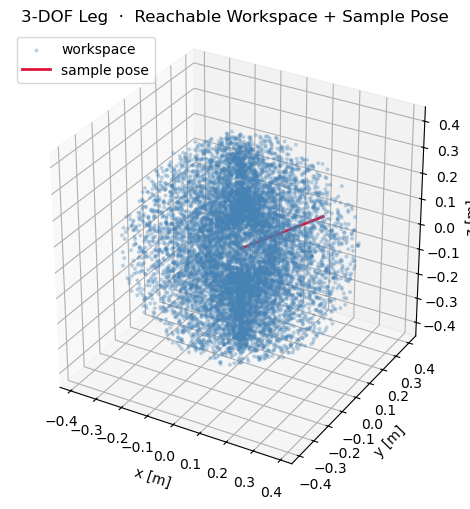
\includegraphics[width=0.9\linewidth]{../figs/exercise_4.png}
  \caption{3-DOF Leg. Reachable Workspace + Sample Pose}
  \label{fig:robotic leg}
\end{figure}

\footnote{Source code and executable notebook available at
\url{https://github.com/Awai005/martian-mindset-mech-control-test/notebooks/Exercise_4_kinematics1.ipynb}}

\newpage

\subsubsection*{Exercise 5}


\text{Vector definitions}

All points lie in the fixed \(xy\)-plane with ground pivot \(O=(0,0)\).

\[
\mathbf l_{1}
   = l_{1}
     \begin{bmatrix}
       \cos q_{1}\\[2pt]
       \sin q_{1}
     \end{bmatrix},
\qquad
\mathbf l_{2}
   = l_{2}
     \begin{bmatrix}
       \cos\phi\\[2pt]
       \sin\phi
     \end{bmatrix},
\qquad
\mathbf d
   =
     \begin{bmatrix}
       d\\[2pt] 0
     \end{bmatrix},
\quad
d=q_{3},
\]

where  

* \(l_{1}\) = crank length \(OA\) (fixed),  
* \(l_{2}\) = connecting-rod length \(AB\) (fixed),  
* \(d\)     = slider displacement \(OB\) (prismatic joint),  
* \(\phi\)  = instantaneous orientation of the rod w.r.t.\ the \(x\)-axis.  

\bigskip

\text{Loop-closure equation}

\[
\;\mathbf l_{1} + \mathbf l_{2} = \mathbf d\;
\]

%%%%%%%%%%%%%%%%%%%%%%%%%%%%%%%%%%%%%%%%%%%%%%%%%%%%%%%%%%%%%%%%%%%%%%%%%%%%
\text{Coordinate form}

\label{eq:loopCoord}
\[
\begin{aligned}
l_{1}\cos q_{1} + l_{2}\cos\phi &= d, \\[2pt]
l_{1}\sin q_{1} + l_{2}\sin\phi &= 0.
\end{aligned}\tag{1}
\]

\text{Eliminating the rod angle \(\phi\)}

Square the two lines of \eqref{eq:loopCoord} and add:

\[
(l_{1}\cos q_{1})^{2} + (l_{1}\sin q_{1})^{2}
  + l_{2}^{2}\!\bigl(\cos^{2}\phi + \sin^{2}\phi\bigr)
  + 2\,l_{1}l_{2}\bigl(\cos q_{1}\cos\phi + \sin q_{1}\sin\phi\bigr)
  = d^{2}.
\]

Because \(\cos^{2}\phi+\sin^{2}\phi = 1\) and  
\(\cos q_{1}\cos\phi + \sin q_{1}\sin\phi = \cos(q_{1}-\phi)\),

\[
l_{1}^{2} + l_{2}^{2} + 2l_{1}l_{2}\cos(q_{1}-\phi) = d^{2}.
\]

Next, express \(\phi\) in terms of \(q_{1}\) and \(d\).
From the second line of \eqref{eq:loopCoord},

\[
\sin\phi = -\frac{l_{1}}{l_{2}}\sin q_{1},
\]
and using \(\cos^{2}\phi+\sin^{2}\phi=1\),

\[
\cos\phi = \frac{d - l_{1}\cos q_{1}}{l_{2}}.
\]

Hence

\[
\cos(q_{1}-\phi)
        = \cos q_{1}\cos\phi + \sin q_{1}\sin\phi
        = \frac{d^{2} - l_{1}^{2} - l_{2}^{2}}{2l_{1}l_{2}}.
\]

Substituting back gives the compact scalar constraint

\begin{align}\label{2}
(d - l_{1}\cos q_{1})^{2} + l_{1}^{2}\sin^{2}q_{1} = l_{2}^{2}
\end{align}

Equation ~\eqref{2} is the fundamental relation linking
the prismatic variable \(d=q_{3}\) and the crank angle \(q_{1}\);
all forward and inverse-kinematics formulas follow directly from it.

\textbf{Forward kinematics  \(\;q_{1}=f(d)\)}

Start from the scalar loop-closure constraint (derived earlier):

\begin{align}\label{1}
(d-l_{1}\cos q_{1})^{2}+l_{1}^{2}\sin^{2}q_{1}=l_{2}^{2}
\end{align}

Expand \eqref{1} and solve for \(\cos q_{1}\):

\[
d^{2}-2l_{1}d\cos q_{1}+l_{1}^{2}=l_{2}^{2}
\;\;\Longrightarrow\;\;
%
\cos q_{1}= \frac{d^{2}+l_{1}^{2}-l_{2}^{2}}{2l_{1}d}
\]

Principal (elbow-up) branch \(q_{1}\in[0,\pi]\):

\[
q_{1}= \arccos\!\Bigl(\tfrac{d^{2}+l_{1}^{2}-l_{2}^{2}}{2l_{1}d}\Bigr)
\]

Reality condition: the $\arccos$ argument must lie in \([-1,1]\), giving the admissible stroke range
\(\bigl|\,l_{1}-l_{2}\bigr|\le d\le l_{1}+l_{2}\).

\textbf{Inverse kinematics  \(\;d=f^{-1}(q_{1})\)}

Re-interpret \eqref{1} as a quadratic in \(d\):

\[
d^{2}-2l_{1}\cos q_{1}\;d + (l_{1}^{2}-l_{2}^{2}) = 0.
\]

Positive (slider-extension) root:

\[%
d = l_{1}\cos q_{1}
    + \sqrt{\,l_{2}^{2}-l_{1}^{2}\sin^{2}q_{1}}\;,
\qquad
|\sin q_{1}|\le\frac{l_{2}}{l_{1}} \;(\text{real stroke}).
\]

\textbf{verification of forward and inverse kinematics}

\begin{figure}[htbp]
  \centering
  % 40 % of text width; keep aspect
  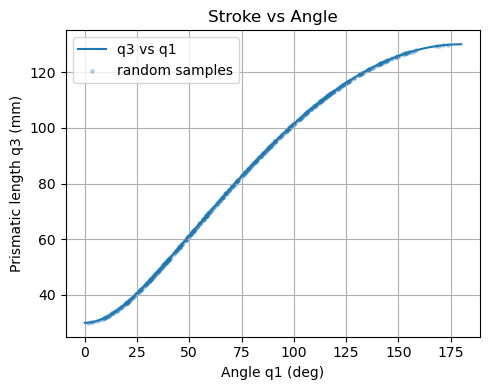
\includegraphics[width=0.9\linewidth]{../figs/exercise_5_1.png}
  \caption{Stroke vs Angle Plot}
  \label{fig:stroke_vs_angle}
\end{figure}


\begin{figure}[htbp]
  \centering
  % 40 % of text width; keep aspect
  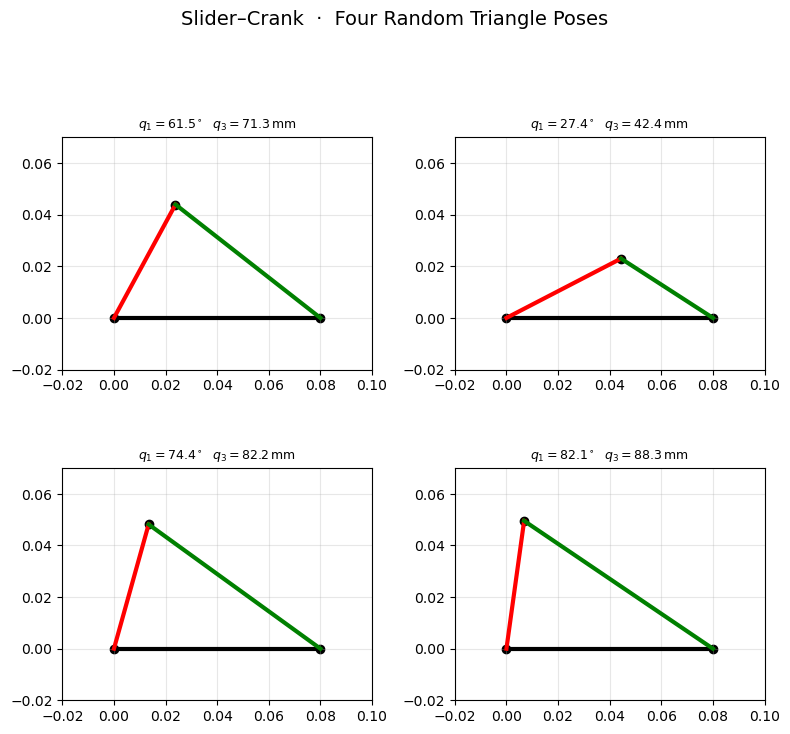
\includegraphics[width=0.9\linewidth]{../figs/exercise_5_2.png}
  \caption{four random Triangle poses}
  \label{fig:slider crank}
\end{figure}

\footnote{Source code and executable notebook available at
\url{https://github.com/Awai005/martian-mindset-mech-control-test/notebooks/Exercise_5_kinematics.ipynb}}




%%%%%%%%%%%%%%%%%%%%%%%%%%%%%%%%%%%%%%%%%%%%%%%%%%%%%%%%%%%%%%%%%%%%%%%%%%%%
\textbf{Jacobian  \(\displaystyle J(d)=\frac{\partial q_{1}}{\partial d}\)}

From the forward relation \(\cos q_{1}=C(d)\) with

\[
C(d)=\frac{d^{2}+l_{1}^{2}-l_{2}^{2}}{2l_{1}d},
\qquad
C'(d)=\frac{\partial C}{\partial d}
      =\frac{1}{2l_{1}}\Bigl(1-\frac{l_{1}^{2}-l_{2}^{2}}{d^{2}}\Bigr),
\]

differentiate \(\cos q_{1}=\cos q_{1}(d)\):

\[
-\sin q_{1}\,\frac{\partial q_{1}}{\partial d}=C'(d)
\quad\Longrightarrow\quad
%
J(d)=\frac{\partial q_{1}}{\partial d}
     =-\frac{1-\displaystyle\frac{l_{1}^{2}-l_{2}^{2}}{d^{2}}}
            {2l_{1}\sin q_{1}}
\]

\textbf{Maximum angular velocity}

With a prismatic speed limit \(\dot d_{\max}\),

\[
\boxed{%
\dot q_{1,\max}
      =\bigl|\,J(d)\bigr|\,\dot d_{\max}
      =\frac{\bigl|1-(l_{1}^{2}-l_{2}^{2})/d^{2}\bigr|}
             {2l_{1}\,|\sin q_{1}|}\;\dot d_{\max}}.
\]

%%%%%%%%%%%%%%%%%%%%%%%%%%%%%%%%%%%%%%%%%%%%%%%%%%%%%%%%%%%%%%%%%%%%%%%%%%%%
\textbf{Maximum output torque}

Virtual–work principle \(f\,\dot d=\tau\,\dot q_{1}\) gives
\(\tau =f/J(d)\).  With actuator force limit \(f_{\max}\):

\[
\boxed{%
\tau_{\max}
      =\frac{f_{\max}}{|J(d)|}
      =\frac{2l_{1}\,|\sin q_{1}|}
             {\bigl|1-(l_{1}^{2}-l_{2}^{2})/d^{2}\bigr|}\;f_{\max}}.
\]




%%%%%%%%%%%%%%%%%%%%%%%%%%%%%%%%%%%%%%%%%%%%%%%%%%%%%%%%%%%%%%%%%%%%%%%%%%%%
\textbf{Singular configurations}
Dead-centre singularities occur at \(q_{1}=0\) or \(\pi\),
where \(\sin q_{1}=0\) and \(|J|\to\infty\), so the mechanism cannot
generate crank torque regardless of actuator force. \cite{Spong2006}.





\subsubsection*{Exercise 6}
\textbf{1} Yes, Angela can find a linear scaling factor to convert the 3D position from meters to inches. The scaling factor is: 
$$k = 39.3701$$
She applies:
$$(x_{B,\text{inches}}, y_{B,\text{inches}}, z_{B,\text{inches}}) = k \cdot (x_{B,\text{meters}}, y_{B,\text{meters}}, z_{B,\text{meters}})$$
and inputs the resulting coordinates into Donald’s model to obtain the actuator commands.

\textbf{2} No, Donald cannot find a single linear scaling factor to convert the 6D pose from Angela’s metric system (meters, quaternions) to his imperial system (inches, Euler angles in degrees). While the translational components can be scaled linearly by $ k = 39.3701 $, the rotational components require a nonlinear transformation from quaternions to Euler angles, followed by a different scaling factor ($ \frac{180}{\pi} $) for degrees. Thus, the conversion is not a single linear scaling across all dimensions.

\textbf{3} Yes, it is possible for Donald and Angela to use each other’s models. Angela converts her base position from meters to inches using the scaling factor $ k = 39.3701 $ and inputs the result into Donald’s model. Donald converts his end-effector position from inches to meters using $ k^{-1} = \frac{1}{39.3701} $ then converts his Euler angles from degrees to radians using $ \frac{\pi}{180} $ and finally transforms the angles to a quaternion using the above equations. The converted pose is then the input into Angela’s model. These conversions are applied externally, respecting the black-box constraint.



\subsection{Dynamics}
\subsubsection*{Exercise 7}

The pendulum is described as follows:
\begin{itemize}
  \item A point mass \( m \) at the end of a massless rod of length \( l \),
  \item Angular displacement \( \theta \) from the vertical (positive counterclockwise),
  \item A revolute joint at the top applying torque \( \tau \).
\end{itemize}

then:
\begin{enumerate}
  \item Torque \( \tau \) in terms of \( \theta, \dot{\theta}, \ddot{\theta} \) (inverse dynamics),
  \item Angular acceleration \( \ddot{\theta} \) in terms of \( \tau \) (forward dynamics).
\end{enumerate}

\textbf{Inverse Dynamics: Expression for Torque}

Lets begin with Newton’s second law for rotational motion:

\[
\tau = I\ddot{\theta} + \text{gravitational torque}
\]

For a point mass \( m \) at distance \( l \), the moment of inertia is:

\[
I = ml^2
\]

The gravitational torque acting on the mass (opposing motion) is:

\[
\tau_g = -mgl\sin\theta
\]

Substituting, we obtain the total torque:

\[
\tau = ml^2\ddot{\theta} + mgl\sin\theta
\]

\text{Final expression:}

\[
\tau = ml^2\ddot{\theta} + mgl\sin\theta
\]

\vspace{1em}

\textbf{Forward Dynamics: Expression for Acceleration}

Rearranging the inverse dynamics equation to solve for \( \ddot{\theta} \):

\begin{align*}
\tau &= ml^2\ddot{\theta} + mgl\sin\theta \\
ml^2\ddot{\theta} &= \tau - mgl\sin\theta \\
\ddot{\theta} &= \frac{\tau - mgl\sin\theta}{ml^2}
\end{align*}

\text{Final expression:}

\[
\ddot{\theta} = \frac{\tau - mgl\sin\theta}{ml^2}
\]

\textbf{Simulation In MATLAB}
\begin{figure}[htbp]
  \centering
  % 40 % of text width; keep aspect
  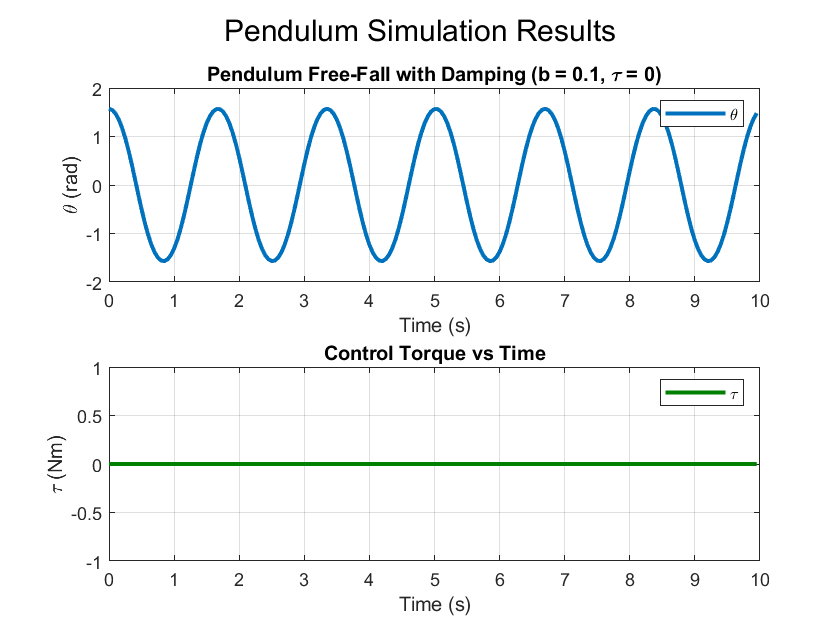
\includegraphics[width=0.9\linewidth]{../figs/exercise_7.png}
  \caption{Free Fall pendulum angle over time}
  \label{fig:slider crank}
\end{figure}
output of angle of pendulum over time. with no damping the system conserves energy and amplitude of oscilation does not change.
\footnote{Source code and executable MATLAB code
\url{https://github.com/Awai005/martian-mindset-mech-control-test/control/Exercise_5_kinematics.ipynb}}


\subsubsection*{Exercise 8}

\textbf{Joint Space Dynamics by Lagrange’s Method}

The joint angles are \( q = [\theta_1, \theta_2]^T \), with velocities \( \dot{q} = [\dot{\theta}_1, \dot{\theta}_2]^T \) and accelerations \( \ddot{q} = [\ddot{\theta}_1, \ddot{\theta}_2]^T \). Link 1 has length \( l_1 \), mass \( m_1 \), and moment of inertia \( I_1 \) about its center of mass (COM) at \( l_1/2 \). Link 2 has length \( l_2 \), mass \( m_2 \), and moment of inertia \( I_2 \) about its COM at \( l_2/2 \). Gravity acts along the negative \( y \)-axis with acceleration \( g \). The coordinate system has the first joint at the origin \((0, 0)\), with the \( x \)-axis horizontal and \( y \)-axis vertical.

\footnote{This solution used below is presented by Asada \cite[Eq.~7-64]{Asada2022}}
\text{Step 1: Kinematics.}
The COM positions are:
\[
x_{c1} = \frac{l_1}{2} \cos \theta_1, \quad y_{c1} = \frac{l_1}{2} \sin \theta_1
\]
\[
x_{c2} = l_1 \cos \theta_1 + \frac{l_2}{2} \cos (\theta_1 + \theta_2), \quad y_{c2} = l_1 \sin \theta_1 + \frac{l_2}{2} \sin (\theta_1 + \theta_2)
\]
Velocities are obtained by time differentiation:
\[
\dot{x}_{c1} = -\frac{l_1}{2} \sin \theta_1 \dot{\theta}_1, \quad \dot{y}_{c1} = \frac{l_1}{2} \cos \theta_1 \dot{\theta}_1
\]
\[
\dot{x}_{c2} = -l_1 \sin \theta_1 \dot{\theta}_1 - \frac{l_2}{2} \sin (\theta_1 + \theta_2) (\dot{\theta}_1 + \dot{\theta}_2)
\]
\[
\dot{y}_{c2} = l_1 \cos \theta_1 \dot{\theta}_1 + \frac{l_2}{2} \cos (\theta_1 + \theta_2) (\dot{\theta}_1 + \dot{\theta}_2)
\]

\text{Step 2: Kinetic Energy.}
The kinetic energy \( T \) includes translational and rotational components for each link. For link 1 (rotating about joint 1, with COM velocity and angular velocity \( \dot{\theta}_1 \)):
\[
T_1 = \frac{1}{2} m_1 (\dot{x}_{c1}^2 + \dot{y}_{c1}^2) + \frac{1}{2} I_1 \dot{\theta}_1^2
\]
\[
\dot{x}_{c1}^2 + \dot{y}_{c1}^2 = \left( \frac{l_1}{2} \sin \theta_1 \dot{\theta}_1 \right)^2 + \left( \frac{l_1}{2} \cos \theta_1 \dot{\theta}_1 \right)^2 = \frac{l_1^2}{4} \dot{\theta}_1^2 (\sin^2 \theta_1 + \cos^2 \theta_1) = \frac{l_1^2}{4} \dot{\theta}_1^2
\]
\[
T_1 = \frac{1}{2} m_1 \cdot \frac{l_1^2}{4} \dot{\theta}_1^2 + \frac{1}{2} I_1 \dot{\theta}_1^2 = \frac{1}{2} \left( \frac{m_1 l_1^2}{4} + I_1 \right) \dot{\theta}_1^2
\]
For link 2 (COM velocity as above, angular velocity \( \dot{\theta}_1 + \dot{\theta}_2 \)):
\[
T_2 = \frac{1}{2} m_2 (\dot{x}_{c2}^2 + \dot{y}_{c2}^2) + \frac{1}{2} I_2 (\dot{\theta}_1 + \dot{\theta}_2)^2
\]
Compute the translational kinetic energy:
\[
\dot{x}_{c2}^2 + \dot{y}_{c2}^2 = \left[ -l_1 \sin \theta_1 \dot{\theta}_1 - \frac{l_2}{2} \sin (\theta_1 + \theta_2) (\dot{\theta}_1 + \dot{\theta}_2) \right]^2 + \left[ l_1 \cos \theta_1 \dot{\theta}_1 + \frac{l_2}{2} \cos (\theta_1 + \theta_2) (\dot{\theta}_1 + \dot{\theta}_2) \right]^2
\]
Expanding and simplifying using trigonometric identities (\( \sin^2 \alpha + \cos^2 \alpha = 1 \), \( \cos (\theta_1 - (\theta_1 + \theta_2)) = \cos (-\theta_2) = \cos \theta_2 \)):
\[
\dot{x}_{c2}^2 + \dot{y}_{c2}^2 = l_1^2 \dot{\theta}_1^2 + \frac{l_2^2}{4} (\dot{\theta}_1 + \dot{\theta}_2)^2 + l_1 l_2 \cos \theta_2 \dot{\theta}_1 (\dot{\theta}_1 + \dot{\theta}_2)
\]
Thus:
\[
T_2 = \frac{1}{2} m_2 \left[ l_1^2 \dot{\theta}_1^2 + \frac{l_2^2}{4} (\dot{\theta}_1 + \dot{\theta}_2)^2 + l_1 l_2 \cos \theta_2 \dot{\theta}_1 (\dot{\theta}_1 + \dot{\theta}_2) \right] + \frac{1}{2} I_2 (\dot{\theta}_1 + \dot{\theta}_2)^2
\]
Total kinetic energy:
\[
T = T_1 + T_2
\]
To express in matrix form \( T = \frac{1}{2} \dot{q}^T M(q) \dot{q} \), collect terms:
\[
T = \frac{1}{2} \left( \frac{m_1 l_1^2}{4} + I_1 + m_2 l_1^2 + \frac{m_2 l_2^2}{4} + I_2 + m_2 l_1 l_2 \cos \theta_2 \right) \dot{\theta}_1^2 + \frac{1}{2} \left( \frac{m_2 l_2^2}{4} + I_2 + \frac{m_2 l_1 l_2}{2} \cos \theta_2 \right) \dot{\theta}_2^2 + \left( \frac{m_2 l_2^2}{4} + I_2 + \frac{m_2 l_1 l_2}{2} \cos \theta_2 \right) \dot{\theta}_1 \dot{\theta}_2
\]
The inertia matrix is:
\[
M(q) = \begin{bmatrix}
I_1 + \frac{m_1 l_1^2}{4} + I_2 + m_2 \left( l_1^2 + \frac{l_2^2}{4} + l_1 l_2 \cos \theta_2 \right) & I_2 + m_2 \left( \frac{l_2^2}{4} + \frac{l_1 l_2}{2} \cos \theta_2 \right) \\
I_2 + m_2 \left( \frac{l_2^2}{4} + \frac{l_1 l_2}{2} \cos \theta_2 \right) & I_2 + \frac{m_2 l_2^2}{4}
\end{bmatrix}
\]

\text{Step 3: Potential Energy.}
The potential energy is:
\[
U = m_1 g y_{c1} + m_2 g y_{c2} = m_1 g \frac{l_1}{2} \sin \theta_1 + m_2 g \left( l_1 \sin \theta_1 + \frac{l_2}{2} \sin (\theta_1 + \theta_2) \right)
\]

\text{Step 4: Lagrangian}
\[
L = T - U
\]

\text{Step 5: Euler-Lagrange Equations.}
For \( \theta_i \ (i=1,2) \):
\[
\tau_i = \frac{d}{dt} \left( \frac{\partial L}{\partial \dot{\theta}_i} \right) - \frac{\partial L}{\partial \theta_i}
\]
- For \( \theta_1 \):
\[
\frac{\partial L}{\partial \dot{\theta}_1} = \frac{\partial T}{\partial \dot{\theta}_1} = M_{11} \dot{\theta}_1 + M_{12} \dot{\theta}_2
\]
\[
\frac{d}{dt} \left( \frac{\partial L}{\partial \dot{\theta}_1} \right) = M_{11} \ddot{\theta}_1 + M_{12} \ddot{\theta}_2 + \dot{M}_{11} \dot{\theta}_1 + \dot{M}_{12} \dot{\theta}_2
\]
\[
\dot{M}_{11} = -m_2 l_1 l_2 \sin \theta_2 \dot{\theta}_2, \quad \dot{M}_{12} = -\frac{m_2 l_1 l_2}{2} \sin \theta_2 \dot{\theta}_2
\]
\[
\frac{\partial L}{\partial \theta_1} = \frac{\partial T}{\partial \theta_1} - \frac{\partial U}{\partial \theta_1}, \quad \frac{\partial T}{\partial \theta_1} = \frac{1}{2} \dot{q}^T \frac{\partial M}{\partial \theta_1} \dot{q}, \quad \frac{\partial M}{\partial \theta_1} = 0
\]
\[
\frac{\partial U}{\partial \theta_1} = m_1 g \frac{l_1}{2} \cos \theta_1 + m_2 g \left( l_1 \cos \theta_1 + \frac{l_2}{2} \cos (\theta_1 + \theta_2) \right)
\]
- For \( \theta_2 \):
\[
\frac{\partial L}{\partial \dot{\theta}_2} = M_{21} \dot{\theta}_1 + M_{22} \dot{\theta}_2
\]
\[
\frac{d}{dt} \left( \frac{\partial L}{\partial \dot{\theta}_2} \right) = M_{21} \ddot{\theta}_1 + M_{22} \ddot{\theta}_2 + \dot{M}_{21} \dot{\theta}_1 + \dot{M}_{22} \dot{\theta}_2, \quad \dot{M}_{21} = -\frac{m_2 l_1 l_2}{2} \sin \theta_2 \dot{\theta}_2, \quad \dot{M}_{22} = 0
\]
\[
\frac{\partial U}{\partial \theta_2} = m_2 g \frac{l_2}{2} \cos (\theta_1 + \theta_2)
\]
Combining terms, the equations are:
\[
\tau = M(q) \ddot{q} + C(q, \dot{q}) \dot{q} + G(q)
\]
where:
\[
G(q) = \begin{bmatrix}
\left( m_1 \frac{l_1}{2} + m_2 l_1 \right) g \cos \theta_1 + m_2 \frac{l_2}{2} g \cos (\theta_1 + \theta_2) \\
m_2 \frac{l_2}{2} g \cos (\theta_1 + \theta_2)
\end{bmatrix}
\]
\[
C(q, \dot{q}) = \begin{bmatrix}
-\frac{m_2 l_1 l_2}{2} \sin \theta_2 \dot{\theta}_2 & -\frac{m_2 l_1 l_2}{2} \sin \theta_2 (\dot{\theta}_1 + \dot{\theta}_2) \\
\frac{m_2 l_1 l_2}{2} \sin \theta_2 \dot{\theta}_1 & 0
\end{bmatrix}
\]

\textbf{Verification}
To verify our analytical derivations for the planar 2R robot arm's joint space dynamics, we developed a MATLAB program using the Symbolic Math Toolbox. The code successfully computes the inertia matrix \( \bm{M}(q) \), Coriolis-centrifugal matrix \( \bm{C}(q, \dot{q}) \), and gravity vector \( \bm{G}(q) \), matching our derived equations perfectly, as shown below:
\footnote{executable MATLAB code here
\url{https://github.com/Awai005/martian-mindset-mech-control-test/control/Exercise_5_kinematics.ipynb}}
\begin{align*}
\bm{M}(q) &= \begin{bmatrix}
I_1 + \frac{m_1 l_1^2}{4} + I_2 + m_2 \left( l_1^2 + \frac{l_2^2}{4} + l_1 l_2 \cos \theta_2 \right) & I_2 + m_2 \left( \frac{l_2^2}{4} + \frac{l_1 l_2}{2} \cos \theta_2 \right) \\
I_2 + m_2 \left( \frac{l_2^2}{4} + \frac{l_1 l_2}{2} \cos \theta_2 \right) & I_2 + \frac{m_2 l_2^2}{4}
\end{bmatrix}, \\
\bm{C}(q, \dot{q}) &= \begin{bmatrix}
-\frac{m_2 l_1 l_2}{2} \sin \theta_2 \dot{\theta}_2 & -\frac{m_2 l_1 l_2}{2} \sin \theta_2 (\dot{\theta}_1 + \dot{\theta}_2) \\
\frac{m_2 l_1 l_2}{2} \sin \theta_2 \dot{\theta}_1 & 0
\end{bmatrix}, \\
\bm{G}(q) &= \begin{bmatrix}
\left( m_1 \frac{l_1}{2} + m_2 l_1 \right) g \cos \theta_1 + m_2 \frac{l_2}{2} g \cos (\theta_1 + \theta_2) \\
m_2 \frac{l_2}{2} g \cos (\theta_1 + \theta_2)
\end{bmatrix}.
\end{align*}

These match our analytical results from Part 1, consistent with \cite[Eqs.~7-44, 7-45]{Asada2022}. To further confirm, we tested the code with numerical values: \( m_1 = m_2 = 1 \, \text{kg} \), \( l_1 = l_2 = 1 \, \text{m} \), \( I_1 = I_2 = \frac{1}{12} \, \text{kg·m}^2 \), \( g = 9.81 \, \text{m/s}^2 \), \( \theta_1 = \theta_2 = \pi/4 \), and \( \dot{\theta}_1 = \dot{\theta}_2 = 0.1 \, \text{rad/s} \). The results are:

\begin{align*}
\bm{M} &\approx \begin{bmatrix} 2.3738 & 0.6869 \\ 0.6869 & 0.3333 \end{bmatrix}, \quad
\bm{C} \approx \begin{bmatrix} -0.0707 & -0.1414 \\ 0.0707 & 0 \end{bmatrix}, \quad
\bm{G} \approx \begin{bmatrix} 10.4051 \\ 0 \end{bmatrix}.
\end{align*}

These numerical values align with manual calculations, and the inertia matrix \( \bm{M} \) is symmetric with positive eigenvalues (0.1237, 2.5835), ensuring it is physically valid. Thus, the MATLAB code confirms our derivations are correct and robust.

\textbf{Operational Space Formulation}

We derive the dynamics in operational space, where the task space coordinates are the end-effector position \( x = [x, y]^T \), and the dynamics take the form:
\[
F = M_x(q) \ddot{x} + C_x(q, \dot{q}) \dot{x} + G_x(q)
\]
with joint torques related by \( \tau = J^T F \).

\text{Step 1: End-Effector Position}
The end-effector is at the tip of link 2:
\[
x = l_1 \cos \theta_1 + l_2 \cos (\theta_1 + \theta_2), \quad y = l_1 \sin \theta_1 + l_2 \sin (\theta_1 + \theta_2)
\]

\text{Step 2: Jacobian Matrix}
The Jacobian \( J \) relates task space velocities \( \dot{x} = [\dot{x}, \dot{y}]^T \) to joint velocities \( \dot{q} \):
\[
\dot{x} = J \dot{q}, \quad J = \begin{bmatrix}
\frac{\partial x}{\partial \theta_1} & \frac{\partial x}{\partial \theta_2} \\
\frac{\partial y}{\partial \theta_1} & \frac{\partial y}{\partial \theta_2}
\end{bmatrix}
\]
\[
\frac{\partial x}{\partial \theta_1} = -l_1 \sin \theta_1 - l_2 \sin (\theta_1 + \theta_2), \quad \frac{\partial x}{\partial \theta_2} = -l_2 \sin (\theta_1 + \theta_2)
\]
\[
\frac{\partial y}{\partial \theta_1} = l_1 \cos \theta_1 + l_2 \cos (\theta_1 + \theta_2), \quad \frac{\partial y}{\partial \theta_2} = l_2 \cos (\theta_1 + \theta_2)
\]
\[
J = \begin{bmatrix}
-l_1 \sin \theta_1 - l_2 \sin (\theta_1 + \theta_2) & -l_2 \sin (\theta_1 + \theta_2) \\
l_1 \cos \theta_1 + l_2 \cos (\theta_1 + \theta_2) & l_2 \cos (\theta_1 + \theta_2)
\end{bmatrix}
\]

\text{Step 3: Operational Space Dynamics}
From joint space dynamics \( \tau = M \ddot{q} + C \dot{q} + G \), we transform to task space. The task space inertia matrix is:
\[
\Lambda(q) = (J M^{-1} J^T)^{-1}
\]
The Coriolis-centrifugal term is:
\[
\mu(q, \dot{q}) = \Lambda J M^{-1} (C \dot{q} - \dot{J} \dot{q})
\]
where \( \dot{J} \) is the time derivative of \( J \), computed by differentiating each element with respect to time. The gravity term is:
\[
p(q) = \Lambda J M^{-1} G
\]
The task space force is:
\[
F = \Lambda \ddot{x} + \mu + p
\]
Joint torques are:
\[
\tau = J^T F = J^T (\Lambda \ddot{x} + \mu + p)
\]
Comparing with \( \tau = M_x \ddot{x} + C_x \dot{x} + G_x \):
\[
M_x(q) = \Lambda, \quad C_x(q, \dot{q}) \dot{x} = \mu, \quad G_x(q) = p
\]
Thus:
\[
F = \Lambda(q) \ddot{x} + \mu(q, \dot{q}) + p(q)
\]
\[
\tau = J^T \big( \Lambda(q) \ddot{x} + \mu(q, \dot{q}) + p(q) \big)
\]

\subsubsection*{Exercise 9}
\textbf{Number of independent scalars in a rigid-body mass–inertia}

Placing the origin at the centre of mass eliminates first moments.  
In $n$-D the spatial inertia is
\(
M=\operatorname{diag}\!\bigl(m,\;I\bigr)
\)
with  

\begin{itemize}
  \item $m$ – one scalar mass,
  \item $I$ – an $n\times n$ symmetric inertia tensor.
\end{itemize}

A real symmetric matrix has $\tfrac{n(n+1)}{2}$ free components
\cite{Murray1994}, so
\[
\#\text{scalars}=1+\tfrac{n(n+1)}{2}.
\]

\begin{center}
\renewcommand{\arraystretch}{1.2}
\begin{tabular}{c|c|l}
$n$ & components & rationale \\ \hline
1 & 1 & only $m$ (no rotation) \\ \hline
2 & 2 & $m$ and one out-of-plane moment $I_{zz}$ \cite[§2.4]{Spong2006} \\ \hline
3 & 7 & $m$ plus six $I_{ij}$ entries \cite[Eq.\,(3.11)]{Featherstone2014}
\end{tabular}
\end{center}

%---------------------------------------------------------------------------
\textbf{Key mathematical property of the mass–inertia matrix}

\[
\boxed{\,M = M^{\!\top} \;>\; 0\,}
\]

That is, $M$ is \emph{symmetric positive-definite}.  
Symmetry ensures power is a legitimate quadratic form;
positive-definiteness guarantees kinetic energy
\(K=\frac12 V^{\!\top}MV>0\) for any non-zero velocity $V$
\cite[§7.2]{Asada2022}.

%---------------------------------------------------------------------------
\textbf{Can Donald and Angela match kinetic energies with one scale factor?}

Yes.  Lengths scale by the constant
\(k = 39.3701\;\text{in}\,\mathrm{m}^{-1}\);
velocities scale by the same $k$, hence  

\[
K_{\text{imperial}}
  = \frac12 \bigl(m\,k^{2}\|v\|^{2}\bigr)
  = k^{2}\,K_{\text{metric}}
  \quad (\text{mass unchanged}).
\]

Because multiplication by $k^{2}$ is linear, a single scalar handles the conversion.

%---------------------------------------------------------------------------
\textbf{Will $M_B$ (base frame) and $M_E$ (tool frame) give the same energy?}

Yes.  Spatial inertias transform as  
\(M_E = X^{-\!\top} M_B X^{-1}\)
with $X$ a $6\times6$ spatial transform
\cite[Eq.\,(3.15)]{Featherstone2014}, and velocities as
\(V_E = X V_B\).  Therefore  

\[
K
  = \tfrac12 V_B^{\!\top} M_B V_B
  = \tfrac12 V_E^{\!\top} M_E V_E,
\]

so both engineers compute identical scalar kinetic energy even though the
matrix representation changes.



\section{Control}
\subsubsection*{Exercise 10}
% Problem 1: Stability Analysis
\text{Stability of Upright Position Without Control}
The pendulum dynamics are:
\[
0.125 \ddot{\theta} + 0.1 \dot{\theta} + 2.4525 \sin \theta = \tau
\]
Without control (\(\tau = 0\)):
\[
\ddot{\theta} = -0.8 \dot{\theta} - 19.62 \sin \theta
\]
In state-space with \(x_1 = \theta - \pi\), \(x_2 = \dot{\theta}\):
\[
\dot{x}_1 = x_2, \quad \dot{x}_2 = -0.8 x_2 + 19.62 \sin x_1
\]
Linearizing at \((x_1, x_2) = (0, 0)\):
\[
\dot{x}_2 \approx 19.62 x_1 - 0.8 x_2
\]
Jacobian:
\[
A = \begin{bmatrix} 0 & 1 \\ 19.62 & -0.8 \end{bmatrix}
\]
Eigenvalues:
\[
\lambda^2 + 0.8 \lambda - 19.62 = 0, \quad \lambda \approx 4.045, -4.845
\]
The positive eigenvalue indicates a saddle point, so the upright position is \textbf{not asymptotically stable}.

\text{PD Controller Design}
The PD controller is:
\[
\tau = -k_p (\theta - \pi) - k_d \dot{\theta}
\]
Dynamics become:
\[
0.125 \ddot{\theta} + (0.1 + k_d) \dot{\theta} + 2.4525 \sin \theta + k_p (\theta - \pi) = 0
\]

% Problem 3: Stability with PD Controller
\textbf{Stability Analysis Using Krasovskii-LaSalle}
Lyapunov function:
\[
V = 0.0625 \dot{\theta}^2 + 2.4525 (1 - \cos \theta) + \frac{1}{2} k_p (\theta - \pi)^2
\]
In state variables:
\[
V = 0.0625 x_2^2 + 2.4525 (1 + \cos x_1) + \frac{1}{2} k_p x_1^2
\]
Derivative:
\[
\dot{V} = -(k_d - 0.1) x_2^2 \leq 0 \quad \text{if } k_d > 0.1
\]
Invariant set where \(\dot{V} = 0\): \(x_2 = 0\):
\[
8 k_p x_1 = 19.62 \sin x_1
\]
Locally, \(x_1 = 0\) if \(k_p \neq 2.4525\). By LaSalle’s principle, the system is \textbf{locally asymptotically stable} at \((\theta, \dot{\theta}) = (\pi, 0)\). Globally, a hybrid controller is needed for swing-up from \((\theta, \dot{\theta}) = (0, 0)\).
The problem asks for stability “from any initial state,” implying global asymptotic stability. However, the pendulum has multiple equilibria ($\theta = k\pi$). Starting from $(\theta, \dot{\theta}) = (0, 0)$, the PD controller may converge to the downward position unless energy is added. To achieve swing-up, an energy-based controller is needed, but for stabilization around $\theta = \pi$, PD is sufficient locally. Globally, a hybrid controller (energy pumping then PD) is implied.

Lets evaluate whether the PD controller designed for the simple pendulum can achieve swing-up from \((\theta, \dot{\theta}) = (0, 0)\) to \((\theta, \dot{\theta}) = (\pi, 0)\) with a torque limit of \(|\tau| \leq 1 \, \text{Nm}\). The pendulum parameters are:
\begin{itemize}
    \item Mass: \(m = 0.5 \, \text{kg}\)
    \item Length: \(l = 0.5 \, \text{m}\)
    \item Gravity: \(g = 9.81 \, \text{m/s}^2\)
    \item Damping: \(b = 0.1 \, \text{Nms/rad}\)
\end{itemize}

The equation of motion, including damping, is:
\[
m l^2 \ddot{\theta} + b \dot{\theta} + m g l \sin \theta = \tau
\]
Substituting the parameters:
\[
0.5 \cdot (0.5)^2 \ddot{\theta} + 0.1 \dot{\theta} + 0.5 \cdot 9.81 \cdot 0.5 \sin \theta = \tau
\]
\[
0.125 \ddot{\theta} + 0.1 \dot{\theta} + 2.4525 \sin \theta = \tau
\]
Solving for \(\ddot{\theta}\):
\begin{equation}
    \ddot{\theta} = \frac{\tau - 0.1 \dot{\theta} - 2.4525 \sin \theta}{0.125} = 8 \tau - 0.8 \dot{\theta} - 19.62 \sin \theta
\end{equation}



The PD controller from Part 1 is:
\[
\tau = -k_p (\theta - \pi) - k_d \dot{\theta}, \quad k_p > 0, \, k_d > 0
\]
With the torque limit \(|\tau| \leq 1 \, \text{Nm}\), the control input is:
\[
\tau = \text{sat} \left( -k_p (\theta - \pi) - k_d \dot{\theta}, 1 \right)
\]
where \(\text{sat}(u, 1) = \max(-1, \min(1, u))\). The dynamics become:
\[
0.125 \ddot{\theta} + 0.1 \dot{\theta} + 2.4525 \sin \theta = \text{sat} \left( -k_p (\theta - \pi) - k_d \dot{\theta}, 1 \right)
\]

% Analysis of PD Controller
\textbf{Does the PD Controller Work?}
To achieve swing-up, the controller must overcome the gravitational potential energy barrier. We analyze the torque requirements and energy dynamics.


The gravitational torque is:
\[
\tau_g = m g l \sin \theta
\]
Maximum at \(\theta = \pm \pi/2\):
\[
\tau_g^{\text{max}} = 0.5 \cdot 9.81 \cdot 0.5 \cdot 1 = 2.4525 \, \text{Nm}
\]
Since \(2.4525 \, \text{Nm} > 1 \, \text{Nm}\), the torque limit restricts the controller’s ability to counter gravity, particularly near \(\theta = \pm \pi/2\).


At \((\theta, \dot{\theta}) = (0, 0)\):
\[
\tau = -k_p (0 - \pi) - k_d \cdot 0 = k_p \pi
\]
For a typical gain \(k_p = 2\):
\[
\tau \approx 2 \cdot 3.1416 \approx 6.2832 \, \text{Nm} > 1 \, \text{Nm}
\]
The torque saturates at \(1 \, \text{Nm}\), limiting the controller’s effectiveness.


The energy required for swing-up is computed as follows:
\begin{itemize}
    \item \textbf{Potential Energy} at \(\theta = 0\):
    \[
    V = m g l (1 - \cos \theta) = 2.4525 (1 - \cos 0) = 0 \, \text{J}
    \]
    \item \textbf{Potential Energy} at \(\theta = \pi\):
    \[
    V = 2.4525 (1 - \cos \pi) = 2.4525 \cdot 2 = 4.905 \, \text{J}
    \]
    \item \textbf{Kinetic Energy}: Zero at both states since \(\dot{\theta} = 0\).
\end{itemize}
Energy difference:
\[
\Delta E = 4.905 - 0 = 4.905 \, \text{J}
\]
The controller must inject \(4.905 \, \text{J}\), but damping (\(b = 0.1\)) dissipates energy via \(-b \dot{\theta}^2\). The power input is:
\[
P = \tau \dot{\theta} \leq 1 \cdot |\dot{\theta}|
\]
With saturation, the PD controller cannot provide sufficient torque to overcome the potential barrier, especially at \(\theta = \pi/2\), where \(\tau_g = 2.4525 \, \text{Nm}\). Thus, the PD controller \textbf{does not work} for swing-up with a 1 Nm torque limit. \footnote{PD controller fails due to torque saturation; swing-up possible with energy-based control}

\textbf{using Energy Levels for swing up}


from Equation \eqref{eq:theta(double)dot}
we get:

\begin{equation}\label{eq:theta(double)dot}
\ddot{\theta} = \frac{\tau - 0.1 \dot{\theta} - 2.4525 \sin \theta}{0.125}
\end{equation}

In state-space form, with state vector \( \mathbf{x} = [\theta, \dot{\theta}]^T = [x_1, x_2]^T \) and input \( u = \tau \):

\begin{equation}
\dot{\mathbf{x}} = \begin{bmatrix} x_2 \\ \frac{u - 0.1 x_2 - 2.4525 \sin x_1}{0.125} \end{bmatrix} = f(\mathbf{x}, u)
\end{equation}

The upright equilibrium is at \( \mathbf{x}_e = [\pi, 0]^T \), \( u_e = 0 \):

\begin{equation}
f([\pi, 0], 0) = \begin{bmatrix} 0 \\ \frac{0 - 0.1 \cdot 0 - 2.4525 \sin \pi}{0.125} \end{bmatrix} = \begin{bmatrix} 0 \\ 0 \end{bmatrix}
\end{equation}

The swing-up strategy uses an energy-based controller until the pendulum’s energy \( E \) exceeds \( 0.9 E_d \), where the desired energy is:

\begin{equation}
E_d = m g l (1 - \cos \pi) = 0.5 \cdot 9.81 \cdot 0.5 \cdot 2 = 4.905 \, \text{J}
\end{equation}

The energy-based controller applies torque:

\begin{equation}
\tau = \text{sat}(-k_e (E - E_d) \dot{\theta}, 1), \quad k_e = 2.0
\end{equation}

When \( E > 0.9 E_d \), it switches to a PD controller:

\begin{equation}
\tau = \text{sat}(-k_p (\theta - \pi) - k_d \dot{\theta}, 1)
\end{equation}

with gains \( k_p = 3.0 \), \( k_d = 0.6 \).

\text{PD gain Design}
The PD gains can be chosen by PD tuning method but since we have a clear model of the plant we derive it somewhat empirically. Let us consider the linearized dynamics around \( \theta = \pi \) (derived fully in Section \ref{sec:lqr}). The linearized system is approximately:

\begin{equation}
\ddot{\theta} \approx 19.62 (\theta - \pi) - 0.8 \dot{\theta} + 8 u
\end{equation}

Applying the PD control \( u = -k_p (\theta - \pi) - k_d \dot{\theta} \):

\begin{equation}
\ddot{\theta} + (0.8 + 8 k_d) \dot{\theta} + (8 k_p - 19.62) (\theta - \pi) \approx 0
\end{equation}

For a stable second-order system \( \ddot{\theta} + 2 \zeta \omega_n \dot{\theta} + \omega_n^2 (\theta - \pi) = 0 \), we aim for critical damping (\( \zeta = 1 \)) and a natural frequency (e.g., \( \omega_n = 5 \, \text{rad/s} \)):

\begin{equation}
\omega_n^2 = 8 k_p - 19.62 = 25 \implies 8 k_p = 44.62 \implies k_p \approx 5.5775
\end{equation}

\begin{equation}
2 \zeta \omega_n = 0.8 + 8 k_d = 10 \implies 8 k_d = 9.2 \implies k_d \approx 1.15
\end{equation}

However, the torque limit constrains the gains. For a deviation \( \theta - \pi = 0.1 \, \text{rad} \):

\begin{equation}
\tau \approx m g l (\theta - \pi) = 2.4525 \cdot 0.1 = 0.24525 \, \text{Nm}
\end{equation}

But at \( \theta - \pi = 0.5 \, \text{rad} \):

\begin{equation}
m g l \sin 0.5 \approx 1.178 \, \text{Nm} > 1 \, \text{Nm}
\end{equation}

Using \( k_p = 5.5775 \), \( k_d = 1.15 \):

\begin{equation}
\tau = -5.5775 \cdot 0.1 - 1.15 \cdot 0.1 = -0.55775 - 0.115 = -0.67275 \, \text{Nm}
\end{equation}

This is within the limit, but for larger deviations, \(\tau\) may exceed 1 Nm. The chosen gains \( k_p = 3.0 \), \( k_d = 0.6 \) reduce the torque:

\begin{equation}
\tau = -3.0 \cdot 0.1 - 0.6 \cdot 0.1 = -0.3 - 0.06 = -0.36 \, \text{Nm}
\end{equation}



\begin{figure}[htbp]
  \centering
  % 40 % of text width; keep aspect
  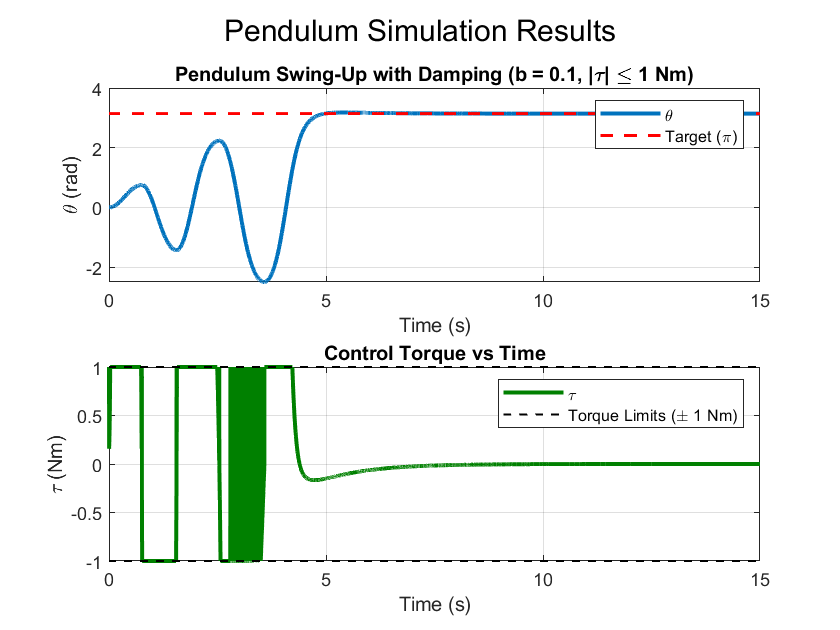
\includegraphics[width=0.9\linewidth]{../figs/pd_swing_up.png}
  \caption{Energy Levels to achieve swing up}
  \label{fig:pd_swing_up}
\end{figure}
The system increases its swinging amptitude gradually until it achieves swing up.

\textbf{Effect of running for twice the time required for swing up}
Running the simulation for a longer period as can be seen in fig. \ref{fig:pd_swing_up}, the pendulum swings up to $\theta \approx \pi$ within 4-6 seconds, then appears to remain stable with $\tau \approx 0$ due to numerical artifacts in the Euler integrator. However, the controller cannot maintain the upright position in a physical sense, as the 1 Nm torque limit is insufficient to counter gravitational torques, and the apparent stability is due to the lack of perturbations and numerical sticking. Performance in the physical sense could be improved by increasing the torque limit, refining gains, using an LQR controller, adding disturbances, or improving the integrator.




\subsubsection*{Exercise 11}\label{sec:lqr}
Here we replace the euler integrator with a Fourth order Runge-Kutta
The following figures represent the plots of angle and torque to time.
\begin{figure}[htbp]
  \centering
  % 40 % of text width; keep aspect
  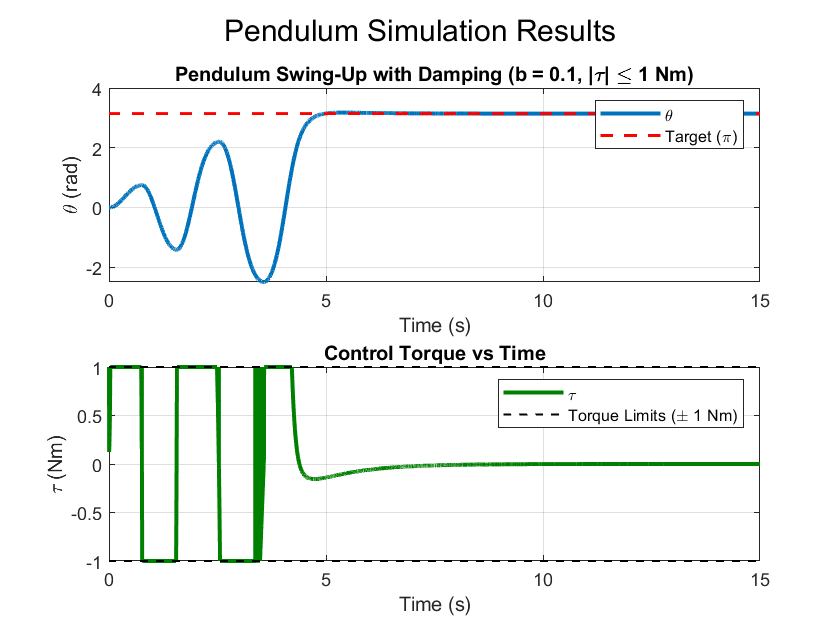
\includegraphics[width=0.9\linewidth]{../figs/rk_pd_swing_up.png}
  \caption{4th order Runge-Kutta integrator with PD controller}
  \label{fig:rk_pd_swing_up}
\end{figure}
\textbf{LQR design}
now lets design a Linear Quadratic regulator:
% Linearizing the dynamics
In Exercise 11, an LQR controller is designed to improve stabilization near \( \theta = \pi \). We linearize the dynamics around the upright equilibrium \( \mathbf{x}_e = [\pi, 0]^T \), \( u_e = 0 \).

The state-space equation is:

\begin{equation}
\dot{\mathbf{x}} = \begin{bmatrix} x_2 \\ \frac{u - 0.1 x_2 - 2.4525 \sin x_1}{0.125} \end{bmatrix} = f(\mathbf{x}, u)
\end{equation}

Define deviation variables \( \tilde{\mathbf{x}} = \mathbf{x} - \mathbf{x}_e = [\theta - \pi, \dot{\theta}]^T \), \( \tilde{u} = u \). Linearize:

\begin{equation}
\dot{\tilde{\mathbf{x}}} \approx A \tilde{\mathbf{x}} + B \tilde{u}
\end{equation}

\[
A = \left. \frac{\partial f}{\partial \mathbf{x}} \right|_{\mathbf{x}_e, u_e}, \quad B = \left. \frac{\partial f}{\partial u} \right|_{\mathbf{x}_e, u_e}
\]

Compute Jacobians:

\[
f_1 = x_2, \quad f_2 = \frac{u - 0.1 x_2 - 2.4525 \sin x_1}{0.125}
\]

\[
\frac{\partial f_1}{\partial x_1} = 0, \quad \frac{\partial f_1}{\partial x_2} = 1
\]

\[
\frac{\partial f_2}{\partial x_1} = \frac{-2.4525 \cos x_1}{0.125}, \quad \frac{\partial f_2}{\partial x_2} = \frac{-0.1}{0.125} = -0.8, \quad \frac{\partial f_2}{\partial u} = \frac{1}{0.125} = 8
\]

Evaluate at \( \mathbf{x}_e = [\pi, 0] \), \( u_e = 0 \):

\[
\frac{\partial f_2}{\partial x_1} = \frac{-2.4525 \cos \pi}{0.125} = \frac{-2.4525 (-1)}{0.125} = 19.62
\]

\[
A = \begin{bmatrix} 0 & 1 \\ 19.62 & -0.8 \end{bmatrix}, \quad B = \begin{bmatrix} 0 \\ 8 \end{bmatrix}
\]

\[
\dot{\tilde{\mathbf{x}}} = \begin{bmatrix} 0 & 1 \\ 19.62 & -0.8 \end{bmatrix} \tilde{\mathbf{x}} + \begin{bmatrix} 0 \\ 8 \end{bmatrix} \tilde{u}
\]

% Designing the LQR controller
The LQR controller minimizes:

\begin{equation}
J = \int_0^\infty \left( \tilde{\mathbf{x}}^T Q \tilde{\mathbf{x}} + \tilde{u}^T R \tilde{u} \right) dt
\end{equation}

Choose \( Q = \begin{bmatrix} 1 & 0 \\ 0 & 1 \end{bmatrix} \) to penalize deviations in \( \theta - \pi \) and \( \dot{\theta} \), and \( R = 1 \) to penalize control effort. Solve the Algebraic Riccati Equation:

\begin{equation}
A^T P + P A - P B R^{-1} B^T P + Q = 0
\end{equation}

\[
R^{-1} = 1, \quad B R^{-1} B^T = \begin{bmatrix} 0 \\ 8 \end{bmatrix} \begin{bmatrix} 0 & 8 \end{bmatrix} = \begin{bmatrix} 0 & 0 \\ 0 & 64 \end{bmatrix}
\]

The gain is:

\begin{equation}
K = R^{-1} B^T P = \begin{bmatrix} 0 & 8 \end{bmatrix} P
\end{equation}

Using MATLAB’s \texttt{lqr} function:

\[
K \approx [2.6646, 0.2042]
\]

The control law is:

\begin{equation}
\tilde{u} = -K \tilde{\mathbf{x}} = -2.6646 (\theta - \pi) - 0.2042 \dot{\theta}
\end{equation}

\[
\tau = \text{sat}(-2.6646 (\theta - \pi) - 0.2042 \dot{\theta}, 1)
\]


\begin{figure}[htbp]
  \centering
  % 40 % of text width; keep aspect
  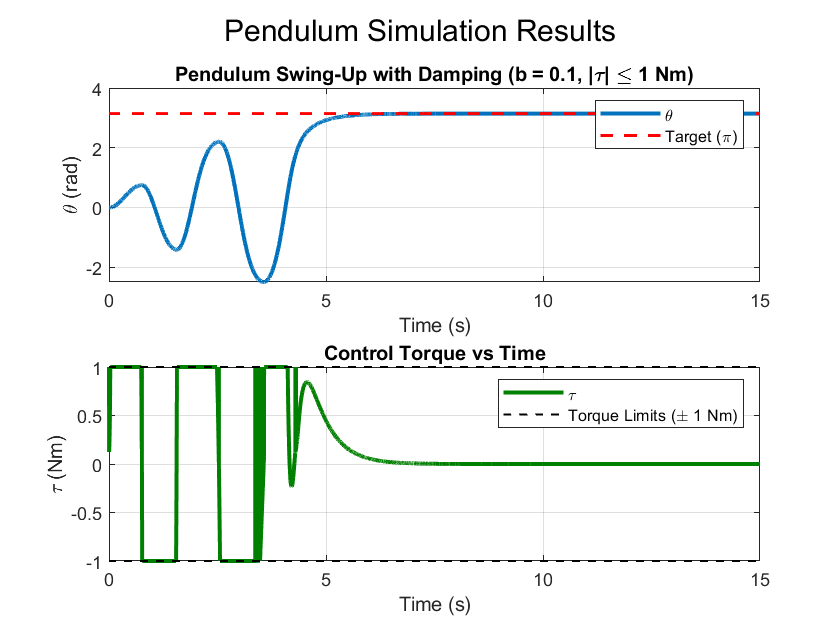
\includegraphics[width=0.9\linewidth]{../figs/lqr_rk_pd_swing_up.png}
  \caption{4th order Runge-Kutta integrator with LQR controller}
  \label{fig:lqr_rk_pd_swing_up}
\end{figure}
\footnote{Since we designed the PD using the Linearized model, it performs almost as well as the LQR controller, however in real life case the presence of perturbations, noise as well as other uncertainties will make the LQR perform better}

\subsubsection*{Exercise 12}
\textbf{Actuator Architectures: Trade-offs and Selection}

\text{Direct-Drive Actuator}

Advantages:
\begin{itemize}
  \item Zero backlash, high torque fidelity and bandwidth.
  \item Direct torque control and intrinsic compliance for impedance control.
\end{itemize}

Disadvantages:
\begin{itemize}
  \item Low torque density—motor must be large.
  \item High rotor inertia.
  \item Costly rare-earth designs.
\end{itemize}


Geared DC Actuator

Advantages:
\begin{itemize}
  \item High torque density via gear reduction.
  \item Compact: small motor + gearbox.
  \item Reflected inertia reduced by gear ratio squared.
\end{itemize}
Disadvantages:
\begin{itemize}
  \item Backlash and stiction—degrades precision.
  \item Limited high-frequency response bandwidth.
  \item Maintenance: lubrication and wear.
\end{itemize}

\text{Series Elastic Actuator (SEA)}

Advantages:
\begin{itemize}
  \item Intrinsic compliance—shock tolerance and safety.
  \item Direct torque measurement via spring deflection.
  \item Robust force control.
\end{itemize}
Disadvantages:
\begin{itemize}
  \item Added mechanical complexity and cost.
  \item Reduced control bandwidth due to elastic dynamics.
\end{itemize}

For our 1Nm swing-up pendulum:
\begin{itemize}
  \item A \emph{geared DC actuator} (10:1) augmented with a small elastic element or strain gauge.
  \item Provides sufficient torque density, moderate bandwidth, low reflected inertia, and built-in torque sensing.
\end{itemize}

\textbf{DC Motor Torque–Speed Characteristic}

\begin{figure}[htbp]
  \centering
  % 40 % of text width; keep aspect
  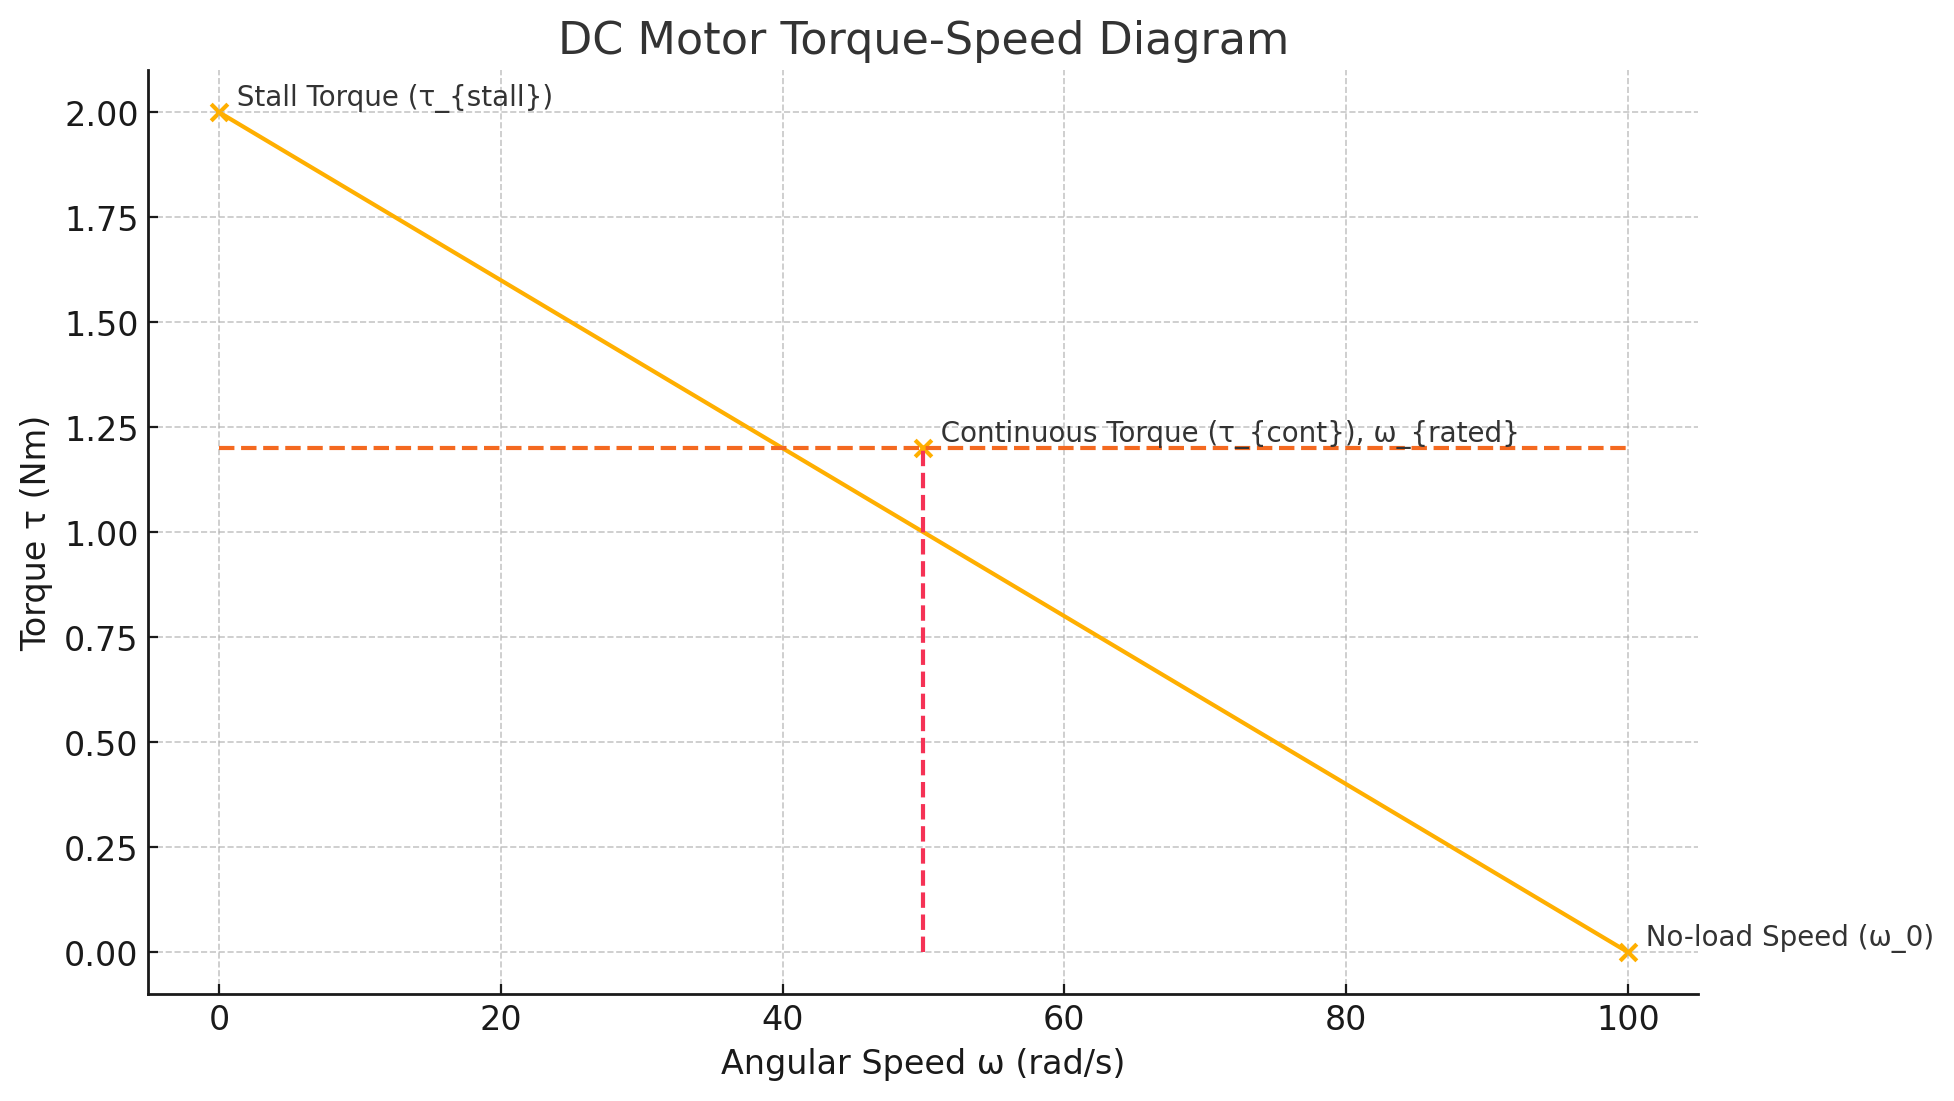
\includegraphics[width=0.9\linewidth]{../figs/output.png}
  \caption{Typical current- and voltage-limited DC motor torque–speed diagram.  
  A gear ratio $r$ scales $\tau_{\rm out} = r\,\tau_{\rm motor}$ and $\omega_{\rm out} = \omega_{\rm motor}/r$.}
  \label{fig:torque_speed}
\end{figure}
When a gear reduction of ratio \(r\) is applied between the motor and the load:
\begin{align*}
  \tau_{\rm out} &= r \,\tau_{\rm motor},   &
  \omega_{\rm out} &= \frac{\omega_{\rm motor}}{r}.
\end{align*}
Graphically, the entire torque–speed line is \emph{stretched} vertically by \(r\) and \emph{compressed} horizontally by \(r\):
\begin{itemize}
  \item Stall torque increases from \(\tau_{\rm stall}\) to \(r\,\tau_{\rm stall}\).
  \item No-load speed decreases from \(\omega_0\) to \(\omega_0/r\).
  \item Continuous torque limit becomes \(r\,\tau_{\rm cont}\), and the rated speed shifts to \(\omega_{\rm rated}/r\).
\end{itemize}
Thus, gearing trades off top speed for higher torque at the output shaft, enlarging the low-speed high-torque region of the operating envelope.


\textbf{Friction and Rotor Inertia in Joint Control}
The joint dynamics with viscous $b_v$ and Coulomb $\tau_c$ friction, and effective inertia $J_{\rm eff}$:
\[
J_{\rm eff}\,\ddot\theta + b_v\,\dot\theta + \tau_c\,\mathrm{sign}(\dot\theta)
+ mgl\sin\theta
= \tau_{\rm cmd}.
\]
\text{Compensation strategies:}
\begin{itemize}
  \item \emph{Inertia feedforward:} $\tau_{\rm ff}=J_{\rm eff}\,\ddot\theta_{\rm des}$.
  \item \emph{Viscous inversion:} $\tau_{\rm ff}=b_v\,\dot\theta_{\rm des}$.
  \item \emph{Coulomb dead-zone:} model stiction and apply $\tau_c\,\mathrm{sign}(\dot\theta_{\rm des})$.
  \item \emph{Torque feedback:} use SEA/strain gauge and close the loop on measured torque.
  \item \emph{Observers:} disturbance observers for unmodeled friction/inertia.
\end{itemize}

\vfill




\bibliographystyle{ieeetr}   % or plain, unsrt, etc.
\bibliography{refs}   
\end{document}
